\section{Training Stability and Collapse}
\label{sec:training}

JEPA-family objectives are non-contrastive: the encoder and predictor
are trained to match a target network's latent output, with no
explicit repulsion between unrelated samples. The known failure mode
is collapse, in which the encoder minimises the loss by mapping every
input to the same point or to a low-rank subspace. A new JEPA
predictor therefore needs evidence that it does not inherit or induce
collapse. This section (i) explains why training loss alone is not a
valid collapse diagnostic for the regularisers used in this
literature, (ii) reports a seed-level collapse phase diagram on a
held-out probe task, and (iii) runs a three-seed $\times$ six-variant
sweep of anti-collapse protocols on UWM-JEPA.

\paragraph{Training loss is not a collapse metric}
VICReg~\cite{bardes2022vicreg}, Barlow Twins~\cite{zbontar2021barlow},
and log-determinant regularisers are hinge-like or barrier-like by
construction. At the optimum the variance, cross-correlation, or
spectral terms sit near their target boundary, so the total training
loss plateaus close to a fixed non-zero value regardless of whether
the encoder has collapsed, and collapsed and healthy encoders can
produce training curves that look nearly identical. Following
standard practice in the JEPA
literature~\cite{assran2023ijepa,assran2024vjepa,caron2021emerging,chen2021exploring,grill2020bootstrap},
collapse is diagnosed downstream: we freeze the encoder after
training, fit a linear probe on a small supervised split, and report
the probe's coefficient of determination on a held-out split. A
non-trivial held-out $R^2$ is direct evidence that the latent space
retains task-relevant structure; a near-zero $R^2$ is direct evidence
of representational collapse regardless of the training loss.

\paragraph{Held-out collapse diagnostic}
Figure~\ref{fig:dashboard} plots the two collapse diagnostics that are
comparable across latent parameterisations: held-out linear-probe $R^2$
and covariance effective rank~\cite{alain2017understanding,roy2007effective}. Each small point is one training seed;
the large marker is the model mean. The shaded region marks the
conservative failure rule used in the experiment ($R^2<0.05$ or
effective rank $<2$). UWM-JEPA and LSTM-JEPA both sit in the
high-probe, non-collapsed region; GRU fails primarily by low rank and
MLP fails by near-zero probe performance despite non-trivial covariance
rank. Pairwise latent distance was computed as an auxiliary diagnostic
but is not plotted because its absolute scale is not comparable between
density-matrix and vector latents.

\begin{figure}[t]
  \centering
  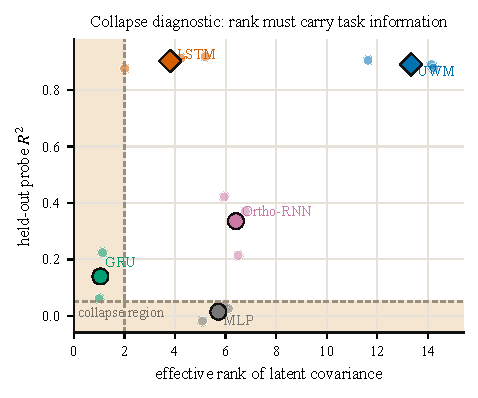
\includegraphics[width=\linewidth]{figures/fig_collapse_phase.pdf}
  \caption{\textbf{Collapse diagnostic on held-out data.}
  Seed-level points compare covariance effective rank against
  linear-probe $R^2$ on hidden velocity. The shaded failure region is
  the conservative collapse rule used in this experiment
  ($R^2<0.05$ or effective rank $<2$)~\cite{roy2007effective}. UWM-JEPA and LSTM-JEPA both
  occupy the non-collapsed, high-probe region; the probe, not the
  training loss, is the primary collapse criterion.}
  \label{fig:dashboard}
\end{figure}

\paragraph{Anti-collapse protocols}
To test whether UWM-JEPA's stability is an artefact of one particular
regulariser, we trained six variants of the UWM-JEPA objective across
three seeds each and evaluated each with the same held-out linear
probe. The variants are: \texttt{none} (stop-gradient target only),
\texttt{contrastive} (InfoNCE-style negatives~\cite{oord2018cpc}), \texttt{ema\_only}
(EMA target network, no explicit regulariser), \texttt{ema\_vicreg}
(EMA plus VICReg), \texttt{ema\_barlow} (EMA plus Barlow Twins), and
\texttt{ema\_logdet} (EMA plus log-determinant penalty).

\begin{table}[t]
  \centering
  \caption{\textbf{Anti-collapse sweep on UWM-JEPA (three seeds per
  variant).} Held-out linear-probe $R^2$ on hidden velocity, mean
  $\pm$ standard deviation. All six variants cross the conservative
  probe threshold on every seed; none of the runs collapsed.}
  \label{tab:multiseed}
  \begin{tabular}{lcc}
    \toprule
    Protocol & Probe $R^2$ mean & Probe $R^2$ std \\
    \midrule
    \texttt{none}          & 0.975 & 0.003 \\
    \texttt{contrastive}   & 0.921 & 0.060 \\
    \texttt{ema\_only}     & 0.975 & 0.003 \\
    \texttt{ema\_vicreg}   & 0.979 & 0.001 \\
    \texttt{ema\_barlow}   & 0.915 & 0.028 \\
    \texttt{ema\_logdet}   & 0.969 & 0.008 \\
    \bottomrule
  \end{tabular}
\end{table}

\paragraph{Scope of the claim}
Every variant in Table~\ref{tab:multiseed} crosses the conservative
probe threshold on every seed, and no run collapsed. The experiment
therefore supports the narrow statement that \emph{UWM-JEPA remained
non-collapsed under the tested protocols in this setting}. Unitarity
does not prevent collapse in general: the theorem in
\cref{sec:theorem} preserves the spectrum of the joint
system--environment state under blind rollout but does not prevent
the encoder from mapping its input to a degenerate joint state in the
first place. Across the regularisers the community typically uses to
rule collapse out, the UWM-JEPA predictor does not re-introduce it.
